%
% teil2.tex -- Beispiel-File für teil2 
%
% (c) 2020 Prof Dr Andreas Müller, Hochschule Rapperswil
%
% !TEX root = ../../buch.tex
% !TEX encoding = UTF-8
%
\section{Einfacher Bruteforce Algorithmus}
In der Bruteforce Methode wird jede Variante durchprobiert, 
um die beste Lösung zu finden. Dabei wird Systematisch ein 
Ablauf durchgemacht und überprüft, wie lange die Strecke ist.
Ist die Strecke kürzer ist dies die neue Optimale Lösung.

\begin{figure} [h]
	\centering
	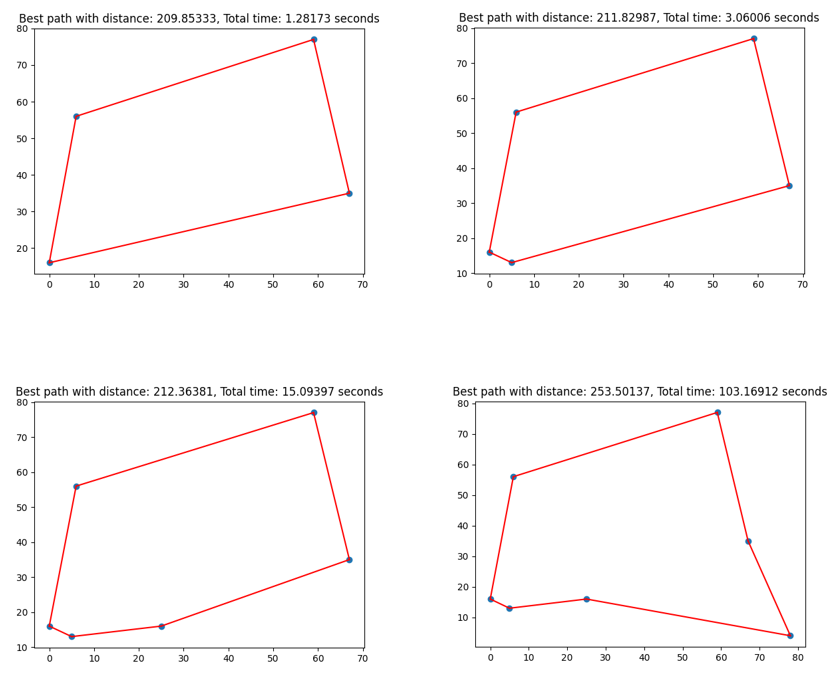
\includegraphics[width=0.8\textwidth]{
        papers/variationsprinzip_algorithmen/images/teil2/02_bruteforce_methode.jpg
        }
	\caption{Abbildung Verschiedener Durchgänge mit steigender Anzahl von Städten}
	\label{fig:Abbildung Verschiedener Durchgänge mit steigender Anzahl von Städten}
\end{figure}

Auf dem Bild ist ersichtlich das mit jedem weiteren Knoten der Aufwand 
exponentiell steigt oder anders ausgedrückt, mit jeder weiteren Knoten
gibt es mehr Variationen, die durchprobiert werden müssen. Die Anzahl 
der Möglichkeiten lässt sich mit der Formel

\begin{equation}
    (n-1)!
\end{equation}

berechnen. Dabei ist \(n\) die Anzahl der Städte.

Die Berechnung der verschiedenen Kombinationen lässt sich mit folgender 
mathematischen Formel beschreiben:

\begin{equation}
    \label{eq:bruteforce_min_formula}
    L(\sigma) = \sum_{i=1}^{n-1} d(\sigma(i), \sigma(i+1)) + d(\sigma(n), \sigma(1))
\end{equation}

Erklärung:\\
- \( L(\sigma) \)  repräsentiert die Gesamtlänge der Rundreise, die durch 
die Permutation \( \sigma \) der Städte definiert ist.\\
- \( \sigma \) ist eine Permutation der Städte \( \{1, 2, \ldots, n\} \),
 (jedes \( \sigma \) hat ein Set mit unterschiedlicher Reihenfolge der Städte).\\
- \( d(i, j) \) die Entfernung zwischen Stadt \( i \) und Stadt \( j \).\\
- \( L(\sigma) \) die Gesamtlänge der Rundreise \( \sigma \).\\

\subsection{Beispiel Rechnung der Formel}
Für Verständnis wie die Formel \ref{eq:bruteforce_min_formula} angewendet wird, 
gibt es hier ein Beispiel, wie diese angewendet wird.

\begin{table}[h]
    \centering
    \begin{tabular}{|c|c|c|c|c|}
    \hline
       & A  & B  & C  & D  \\ \hline
    A  & 0  & 10 & 15 & 20 \\ \hline
    B  & 10 & 0  & 35 & 25 \\ \hline
    C  & 15 & 35 & 0  & 30 \\ \hline
    D  & 20 & 25 & 30 & 0  \\ \hline
    \end{tabular}
    \caption{Beispiel Tabele mit möglicher Distanz der Städten}
    \label{tab:example_bruteforce_cities}
\end{table}
    
In der Beispiel Tabelle \ref{tab:example_bruteforce_cities} sind die Distanzen zwischen den Städten A, B, C und D aufgeführt.
Zu Lesen ist beispielsweise, dass die Distanz zwischen Stadt B und D 25 beträgt.

Eine mögliche Permutation wäre \(\sigma = (A, B, C, D)\) oder \(\sigma = (B, D, A, C)\).

Die Permutation \(\sigma = (B, D, A, C)\) wird nun in die Formel \ref{eq:bruteforce_min_formula} eingesetzt.

In der Formel \ref{eq:bruteforce_min_formula} wird nun die Distanz zwischen den Städten berechnet.

\begin{equation}
    \label{eq:bruteforce_min_formula}
    L(\sigma) = \sum_{i=1}^{n-1} d(\sigma(i), \sigma(i+1))
\end{equation}

Mit \( L(\sigma(1)) \) würde aus dem Set das B genommen und das führt dann zu dieser aufstellung
\begin{equation}
    \label{eq:bruteforce_min_formula}
        L_1 = d(B, D) + d(D, A) + d(A, C) + d(C, B)
            = 25 + 20 + 15 + 35 = 95
\end{equation}
Dann werden alle mögliche Kombinationen durchgerechnet und die kürzeste Strecke wird als Lösung genommen.

\subsection{Aufwand}
Aus den Vorherigen Abschnitten ist ersichtlich, dass der Aufwand für die Berechnung der kürzesten Strecke
exponentiell steigt. Mit jedem weiteren Knoten gibt es mehr Variationen, die durchprobiert werden müssen.

\subsection{Bruteforce Script}
Das ganze Bruteforce Verfahren gibt es als Script in der Programmiersprache Python auf github 
\footnote{\url{https://github.com/feiler/math_sem_algorithm_variation_principle}}
\cite{algorythm:repo}
herutnerzuladen und selbstzu test.


